\documentclass[10pt]{scrartcl}

\usepackage[utf8]{inputenc}
\usepackage{tabularx}
\usepackage[ngerman]{babel}
\usepackage[automark]{scrpage2}
\usepackage{amsmath,amssymb,amstext}
%\usepackage{mathtools}
\usepackage[]{color}
\usepackage[]{enumerate}
\usepackage{graphicx}
\usepackage{lastpage}
\usepackage[perpage,para,symbol*]{footmisc}
\usepackage{listings} 
\usepackage[pdfborder={0 0 0},colorlinks=false]{hyperref}
\usepackage[numbers,square]{natbib}
\usepackage{color}
\usepackage{colortbl}
\usepackage{listings}
\usepackage{a4wide}
\usepackage{xspace}
\usepackage{listings}
\usepackage{hyperref}
\usepackage{epstopdf}

\lstset{numbers=left, numberstyle=\tiny, numbersep=5pt, breaklines=true, showstringspaces=false} 

%changehere
\def\titletext{TH1 Praktikum 3 : Ausarbeitung}
\def\titletextshort{Praktikum 3}
\author{Carsten Noetzel, Armin Steudte}

\title{\titletext}

%changehere Datum der Übung
\date{16.05.2012}

\pagestyle{scrheadings}
%changehere
\ihead{TH1, Padberg}
\ifoot{Generiert am:\\ \today}

\cfoot{Carsten Noetzel, Armin Steudte}


\ohead[]{\titletextshort}
\ofoot[]{{\thepage} / \pageref{LastPage}}

\setlength{\parindent}{0.0in}
\setlength{\parskip}{0.1in}

\begin{document}
\maketitle

\setcounter{tocdepth}{3}
\tableofcontents
\listoffigures
%\lstlistoflistings

\section{Aufgabe 1}
\begin{enumerate}
\item{Reversibilität / Lebendigkeit}\\
Lebendigkeit $\Rightarrow$ Reversibilität, da aus der Lebendigkeit folgt, dass es eine echt positive T-Invariante gibt für die gilt $\forall t \in T : I_{T}(t) \geq 1$. Weiterhin setzt ein lebendiges Netz voraus, dass alle $t \in T$  M-aktiviert sind, wodurch man von einer beliebigen Markierung M aus jede Transition erreichen können muss.\\
Die Umkehrung gilt nicht! Reversibilität $\nRightarrow$ Lebendigkeit

\item{Beschränktheit / Lebendigkeit}\\
Zwischen der Beschränktheit eines Netzes und seiner Lebendigkeit gibt es keinen direkten Zusammenhang. Ein Netz kann beschränkt und lebendig (Abbildung \ref{fig:BL}), beschränkt und nicht lebendig (Abbildung \ref{fig:BnL}), unbeschränkt und lebendig (Abbildung \ref{fig:nBL}) und unbeschränkt und nicht lebendig sein (Abbildung \ref{fig:nBnL}).

\begin{figure}
\begin{minipage}[hbt]{7cm}
	\centering
	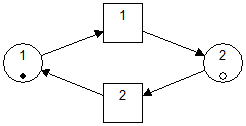
\includegraphics[width=0.7\textwidth]{Bilder/2_Beschraenkt_und_Lebendig.png}
	\caption{beschränktes und lebendiges Netz}
	\label{fig:BL}
\end{minipage}
\hfill
\begin{minipage}[hbt]{7cm}
	\centering
	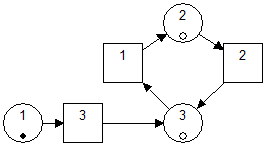
\includegraphics[width=0.7\textwidth]{Bilder/2_Beschraenkt_nicht_Lebendig.png}
	\caption{beschränktes und nicht lebendiges Netz}
	\label{fig:BnL}
\end{minipage}
\end{figure}
\begin{figure}
\begin{minipage}[hbt]{7cm}
	\centering
	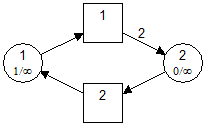
\includegraphics[width=0.7\textwidth]{Bilder/2_Nicht_Beschraenkt_und_Lebendig.png}
	\caption{unbeschränktes und lebendiges Netz}
	\label{fig:nBL}
\end{minipage}
\hfill
\begin{minipage}[hbt]{7cm}
	\centering
	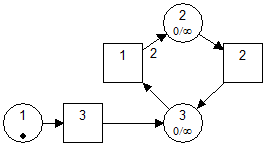
\includegraphics[width=0.7\textwidth]{Bilder/2_Nicht_Beschraenkt_nicht_Lebendig.png}
	\caption{unbeschränktes und nicht lebendiges Netz}
	\label{fig:nBnL}
\end{minipage}
\end{figure}

\item{Beschränktheit / Reversibilität}\\
Zwischen Beschränktheit und Reversibilität eines Netzes gibt es keinen direkten Zusammenhang. Ein Netz kann beschränkt und reversibel (Abbildung \ref{fig:BR}), beschränkt und nicht reversibel (Abbildung \ref{fig:BnR}), unbeschränkt und reversibel (Abbildung \ref{fig:nBR}) und unbeschränkt und nicht reversibel sein (Abbildung \ref{fig:nBnR}).


\begin{figure}
\begin{minipage}[hbt]{7cm}
	\centering
	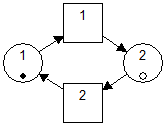
\includegraphics[width=0.7\textwidth]{Bilder/3_beschraenkt_und_reversibel.png}
	\caption{beschränktes und reversibles Netz}
	\label{fig:BR}
\end{minipage}
\hfill
\begin{minipage}[hbt]{7cm}
	\centering
	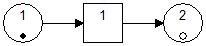
\includegraphics[width=0.7\textwidth]{Bilder/3_beschraenkt_nicht_reversibel.png}
	\caption{beschränktes und nicht reversibles Netz}
	\label{fig:BnR}
\end{minipage}
\end{figure}
\begin{figure}
\begin{minipage}[hbt]{7cm}
	\centering
	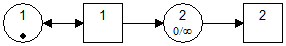
\includegraphics[width=0.7\textwidth]{Bilder/3_unbeschraenkt_und_reversibel.png}
	\caption{unbeschränktes und reversibles Netz}
	\label{fig:nBR}
\end{minipage}
\hfill
\begin{minipage}[hbt]{7cm}
	\centering
	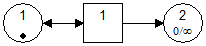
\includegraphics[width=0.7\textwidth]{Bilder/3_unbeschraenkt_nicht_reversibel.png}
	\caption{unbeschränktes und nicht reversibles Netz}
	\label{fig:nBnR}
\end{minipage}
\end{figure}

\item{Erreichbarkeit / Lebendigkeit}\\
Lebendigkeit $\Rightarrow$ Erreichbarkeit\\
Wenn ein $t \in T$ lebendig ist, muss es $\forall M \in EG$ M-erreichbar sein, daraus folgt $\exists M \in EG$ für das gilt t ist aus M erreichbar.\\
Wenn das Netz lebendig ist, sind alle Transitionen lebendig und damit $\forall M \in EG$ M-erreichbar.

\item{Erreichbarkeit / Reversibilität}\\
Reversibilität $\Rightarrow$ Erreichbarkeit\\
Wenn ein Netz reversibel ist, muss es einen Weg von $M_{0} \overset{*}{\rightarrow} M \overset{*}{\rightarrow} M_{0}$ geben, somit gilt: $\forall t \in T$ sind von jeder $M \in EG$ M-erreichbar.
Die Umkehrung gilt nicht! Erreichbarkeit $\nRightarrow$ Reversibilität

\item{Erreichbarkeit / Beschränktheit}\\
\label{erreichbarkeit_beschraenktheit}
Es gibt keinen Zusammenhang. Da die Erreichbarkeit $\forall t \in T$ ein notwendiges Kriterium dafür ist, dass ein Netz lebendig ist, kann an dieser Stelle auf die Beispiele aus Punkt 2 verwiesen werden.\\
Ein Netz kann beschränkt sein und alle $t \in T$ sind erreichbar (lebendig) (Abbildung \ref{fig:BL}), beschränkt und nicht alle $t \in T$ sind erreichbar (nicht lebendig) (Abbildung \ref{fig:BnL}), unbeschränkt und alle $t \in T$ sind erreichbar (lebendig) (Abbildung \ref{fig:nBL}) und unbeschränkt und nicht alle $t \in T$ sind erreichbar (nicht lebendig) sein (Abbildung \ref{fig:nBnL}).

\item{Stelleninvarianten / Lebendigkeit}\\
Stelleninvarianten sagen etwas über die Beschränktheit von Netzen aus. Da bereits gezeigt wurde, dass es keinen Zusammenhang zwischen Beschränktheit und Lebendigkeit gibt, sei hier auf die Beispiele aus Punkt 2 verwiesen.\\
Für die beschränkten Netze aus Abbildung \ref{fig:BL} und \ref{fig:BnL} gibt es Stelleninvarianten, für die unbeschränkten Netze aus Abbildung \ref{fig:nBL} und \ref{fig:nBnL} gibt es keine Stelleninvarianten unabhängig davon ob das Netz lebendig ist oder nicht.

\item{Stelleninvarianten / Reversibilität}\\
Es gibt keinen direkten Zusammenhang. Gibt es keine Stelleninvariante ist das Netz unbeschränkt und kann sowohl reversibel als auch nicht reversibel sein. Hierzu sei auf die Beispiele von Punkt 3 verwiesen.

\item{Stelleninvarianten / Beschränktheit}\\
$\forall p \in P$ $I_{P}(p) > 0$ und $I_{P}(p')\geq 0$ $\forall p' \in P$ $\Rightarrow$ p ist beschränkt\\
Gehören alle $p \in P$ einer solchen positiven Stelleninvariante an $\Rightarrow$ Netz ist beschränkt\\
Die Umkehrung gilt nicht! Beschränktheit $\nRightarrow$ $\forall p \in P$ gehören positiver Stelleninvariante an

\item{Stelleninvarianten / Erreichbarkeit}\\
Die Stelleninvariante trifft Aussagen bezüglich der Beschränktheit eines Netzes.
Wie bereits unter dem Punkt \ref{erreichbarkeit_beschraenktheit} diskutiert wurde, existiert zwischen Beschränktheit und Erreichbarkeit kein direkter Zusammenhang.
Hierbei sei auch auf die unter dem Punkt referenzierten Beispiele verwiesen.

\item{Transitionsinvarianten / Lebendigkeit}\\
Zwischen der Transitionsinvariante und Lebendigkeit existiert der Zusammenhang, dass Lebendigkeit $\Rightarrow$ pos. Transitionsinvariante.\\
Da $N_{M0}$ lebendig ist, wenn $\forall t \in T$ lebendig sind.
Eine Transition $t \in T$ ist lebendig, wenn sie für alle $M \in EG$ M-erreichbar ist.
Somit beschreibt die Transitionsinvariante den Zyklus, dass wenn $t$ geschaltet hat es durch geforderte M-Rrreichbarkeit auch wieder schalten kann. 

\item{Transitionsinvarianten / Reversibilität}\\
Wenn $N_{M0}$ reversibel ist $\exists$ T-Invariante, da es einen Zyklus von $M_{0} \overset{*}{\rightarrow} M  \overset{*}{\rightarrow} M_{0}  \forall M \in EG$ für Reversibilität geben muss.

\item{Transitionsinvarianten / Beschränktheit}\\
Die Beschränktheit stellt eine notwendige Bedingung für das Vorliegen einer Transitionsinvariante dar.
Ohne Beschränktheit kann es kein Transitionsinvariante geben, da man von einem beliebigen Markierung dann nicht mehr zur gleichen Markierung im EG zurückkommen kann.
Es existiert damit keine Schaltsequenz $M \overset{*}{\rightarrow} M$.

\item{Transitionsinvarianten / Erreichbarkeit}\\
Wie bereits erwähnt folgt aus Lebendigkeit $\Rightarrow$ pos. Transitionsinvariante und Lebendigkeit $\Rightarrow$ Erreichbarkeit. 
Da für die Lebendigkeit eines Netzes $N_{M0}$ M-Erreichbarkeit $\forall t \in T$ vorausgesetzt wird und aus Lebendigkeit auf das Vorhandensein einer pos. Transitionsinvariante geschlossen werden kann gilt: Positive Transitionsinvariante $\Leftarrow$ Lebendigkeit $\Rightarrow$ Erreichbarkeit.

\item{Transitionsinvarianten / Stelleninvarianten}\\
Damit eine Transitionsinvariante existieren kann muss das Netzt $N$ mindestens aus einer Transition und einer Stelle bestehen (die Stelle $p_{1}$ stellt die Vor- und Nachbedingung von $t_{1}$ in diesem Fall dar, $\bullet t_{1} = \{p_{1}\}$ und $t_{1} \bullet = \{p_{1}\}$ ).\\
Da mit dem Vorhandensein einer Stelle auch eine Stelleninvariante existiert gilt: $\exists Transitionsinvariante \Rightarrow \exists Stelleninvariante$

\item{Überdeckungsgraph / Lebendigkeit}\\
Lebendigkeit baut auf dem EG auf. Ist eine Transition $t \in T$ im EG M-erreichbar, so ist sie auch im UG M-erreichbar.
Somit ist ein Netz $N$ welches im EG lebendig ist auch im UG lebendig.

\item{Überdeckungsgraph / Reversibilität}\\
$\exists \omega$-Markierung im UG $\Rightarrow$ EG ist unendlich $\Rightarrow$ Netz ist nicht reversibel, da keine Schaltsequenz $M_{0} \overset{*}{\rightarrow} M_{0}$ existiert.

\item{Überdeckungsgraph / Beschränktheit}\\
Sind UG und EG identische (keine $\omega$-Markierungen im UG) $\Rightarrow$ das Netz $N$ ist beschränkt.
$\exists \omega$-Markierung im UG $\Rightarrow$ Netz $N$ ist unbeschränkt.

\item{Überdeckungsgraph / Erreichbarkeit}\\
Ist eine Transition im EG M-erreichbar, so ist sie auch im UG M-erreichbar. $\exists M \in EG \Rightarrow M \in UG$ ggf. überdeckt durch $\omega$-Markierung.

\item{Überdeckungsgraph / Stelleninvarianten}\\
$\exists$ P-Invariante dann ist das Netz $N$ beschränkt. 
Wenn das Netz beschränkt ist sind EG und UG identisch.
Das bedeutet: $\exists$ P-Invariante $\Rightarrow$ EG=UG.

\item{Überdeckungsgraph / Transitionsinvarianten}\\
$\exists$ T-Invariante so gibt es einen Zyklus EG.
Somit existiert dieser Zyklus auch im UG.

\item{Kondensation des EG / Lebendigkeit}\\
\label{eg_lebendigkeit}
Besitz der KG des EG mehr als einen Knoten so ist das Netz nicht lebendig, da die Transition t, die zwischen zwei Knoten im Kg schaltet, nicht M-erreichbar ist.\\
Somit kann die Bedingung für Lebendigkeit ($\forall t \in T$, $t$ ist M-erreichbar) nicht erfüllt sein.

\item{Kondensation des EG  / Reversibilität}\\
Besitzt eine KG mehr als einen Knoten $\Rightarrow$ das Netz $N$ ist nicht reversibel, da ein Reversibles Netz von jeder Markierung M im EG nach $M_{0}$ schalten kann und somit zu einem Knoten im KG zusammenfällt. 

\item{Kondensation des EG  / Beschränktheit}\\
Um einen KG aufbauen zu können muss das Netz beschränkt sein. 
Der EG eines unbeschränkten Netzes ist unendlich, wodurch sich kein KG erstellen lässt. 

\item{Kondensation des EG  / Erreichbarkeit}\\
KG hat mehr als einen Knoten $\Rightarrow$ nicht alle $t \in T$ sind M-erreichbar (vgl. \ref{eg_lebendigkeit}).

\item{Kondensation des EG  / Stelleninvarianten}\\
Zwischen der Kondensation des EG (KG) und den Stelleninvarianten eines Netzes gibt es keinen direkten Zusammenhang. 
Ein Netz muss beschränkt sein, damit der KG erzeugt werden kann, was bei unbeschränkten Netzen nicht der Fall ist. Daraus folgt:\\
Netz ist unbeschränkt $\Rightarrow$ EG kann nicht erzeugt werden.

\item{Kondensation des EG  / Transitionsinvarianten}\\
Zwischen der Kondensation des EG (KG) und den Transitionsinvarianten eines Netzes gibt es keinen Zusammenhang. Zwar zeigen die einzelnen Komponenten des KG Zyklen des Netzes, doch können diese Komponenten auch Senken im Netz sein. Das ist allein aus den Komponenten nicht ersichtlich. Verwiesen sei hier auch die Beispiele von Punkt 36 bei dem wir sowohl Netze mit als auch ohne Transitionsinvarianten haben (Abbildung \ref{fig:VKGN} und \ref{fig:nVKGN}) und die KGs gleich aussehen.

\item{Kondensation des EG  / Überdeckungsgraph}\\
Die Kondensation des EG (KG) und der Überdeckungsgraph (UG) bauen beide auf dem Erreichbarkeitsgraphen (EG) des Netzes auf. Der UG wird genutzt um endliche Netze zu erhalten, wenn der EG eines Netzes aufgrund der Unbeschränktheit unendlich groß wird und der KG zeigt Zyklen im Netz auf und fasst diese zu Komponenten zusammen.

\item{Verklemmung / Lebendigkeit}\\
Verklemmung $\Rightarrow$ nicht lebendig\\
Für die Lebendigkeit eines Netzes gilt $\forall t \in T$ sind M-Erreichbar, d.h. man kann von jeder Markierung $M \in EG$ jede Transition irgendwann einmal schalten. Da wird bei einer Verklemmung in einen Zustand M gelangen in dem keine Transition mehr aktiviert ist, wird die Bedingung für die Lebendigkeit nicht erfüllt und das Netz kann nicht lebendid sein.
Die Umkehrung gilt nicht! nicht lebendig $\nRightarrow$ Verklemmung

\item{Verklemmung / Reversibilität}\\
Verklemmung $\Rightarrow$ nicht reversibel\\
Gelangt das Netz in einen Zustand in dem es keine aktivierten Transitionen mehr gibt, liegt eine Verklemmung vor. Da keine Transition mehr schalten kann, hat das Netz keine Möglichkeit wieder in seinen Ursprungszustand zurückzukehren. Die Bedingung $M_{0} \overset{*}{\rightarrow} M \overset{*}{\rightarrow} M_{0}$ für die Reversibilität ist verletzt.

\item{Verklemmung / Beschränktheit}\\
Zwischen Verklemmung und Beschränktheit gibt es keinen Zusammenhang. An dieser Stelle sei auf die Beispiele aus Punkt 34 verwiesen. Dort ist ein beschränktes Netz mit Verklemmung (Abbildung \ref{fig:SV}) und ohne Verklemmung (Abbildung \ref{fig:SoV}), sowie ein unbeschränktes Netz mit Verklemmung (Abbildung \ref{fig:oSV}) und ohne Verklemmung (Abbildung \ref{fig:oSoV}) dargestellt.

\item{Verklemmung / Erreichbarkeit}\\
Es gilt Verklemmung $\Rightarrow$ Netz ist nicht lebendig (siehe Punkt 29) und aus dieser nicht Lebendigkeit des Netzes folgt: $\exists t \in T$ für das Gilt t ist nicht M-Erreichbar. Durch diese transitive Abhängigkeit lässt sich folgern:\\
Verklemmung $\Rightarrow$ $\exists t \in T :\text{t ist nicht M-Erreichbar}$

\item{Verklemmung / Stelleninvarianten}\\
Zwischen Stelleninvarianten und Verklemmungen gibt es keinen Zusammenhang. Man kann sowohl ein Netz bauen, das eine Stelleninvariante besitzt und eine Verklemmung hat (Abbildung \ref{fig:SV}), keine Stelleninvariante besitzt und eine Verklemmung hat (Abbildung \ref{fig:oSV}) oder mit Stelleninvariante verklemmungsfrei ist (Abbildung \ref{fig:SoV}) bzw. ohne Stelleninvariante verklemmungsfrei ist (Abbildung \ref{fig:oSoV}).

\begin{figure}
\begin{minipage}[hbt]{7cm}
	\centering
	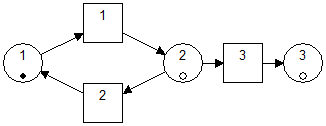
\includegraphics[width=0.7\textwidth]{Bilder/33_Stelleninvariante_mit_Verklemmung.png}
	\caption{Netz mit S-Invariante und mit Verklemmung}
	\label{fig:SV}
\end{minipage}
\hfill
\begin{minipage}[hbt]{7cm}
	\centering
	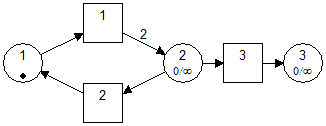
\includegraphics[width=0.7\textwidth]{Bilder/33_ohne_Stelleninvariante_mit_Verklemmung.png}
	\caption{Netz ohne S-Invariante und mit Verklemmung}
	\label{fig:oSV}
\end{minipage}
\end{figure}
\begin{figure}
\begin{minipage}[hbt]{7cm}
	\centering
	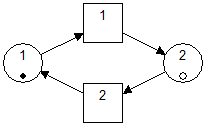
\includegraphics[width=0.7\textwidth]{Bilder/33_Stelleninvariante_ohne_Verklemmung.png}
	\caption{Netz mit S-Invariante und ohne Verklemmung}
	\label{fig:SoV}
\end{minipage}
\hfill
\begin{minipage}[hbt]{7cm}
	\centering
	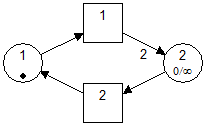
\includegraphics[width=0.7\textwidth]{Bilder/33_ohne_Stelleninvariante_ohne_Verklemmung.png}
	\caption{Netz ohne S-Invariante und ohne Verklemmung}
	\label{fig:oSoV}
\end{minipage}
\end{figure}

\item{Verklemmung / Transitionsinvarianten}\\
Liegt eine positive Transitionsinvariante vor, so gilt $\forall t \in T : I_{T}(t)\geq1$. Das heißt alle Transitionen schalten mindestens einmal. Daraus folgt, dass auch die Transition die zu einer Verklemmung führen müsste schaltet. Da die Transitionsinvariante jedoch Zyklen im Netz beschreibt, kann es nicht zu keiner Verklemmung kommen, da die T-Invariante beliebig oft schalten kann.\\
positive T-Invariante $\Rightarrow$ keine Verklemmung 

\item{Verklemmung / Überdeckungsgraph}\\
Wenn $\exists M \in UG$ für das gilt $\forall t \in T$ sind nicht aktiviert $\Rightarrow$ Verklemmung\\
Gibt es im UG eine Markierung M für die gilt, dass keine Transition aktiviert ist und schalten kann, liegt eine Verklemmung vor und der Zustand kann nicht mehr verlassen werden.

\item{Verklemmung / Kondensation des EG}\\
Man kann dem kondensierten Erreichbarkeitsgraphen eines Netzes nicht ansehen, ob das Netz verklemmt ist oder nicht. Abbildung \ref{fig:VKGN} zeigt ein Netz mit Verklemmung und den dazugehörigen KG in Abbildung \ref{fig:VKGG}. Dieser KG ähnelt dem des nicht verklemmten Netzes aus Abbildung \ref{fig:nVKGN} mit dem KG aus Abbildung \ref{fig:nVKGG}.

\begin{figure}
\begin{minipage}[hbt]{7cm}
	\centering
	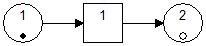
\includegraphics[width=0.7\textwidth]{Bilder/36_Verklemmung_KG_Netz.png}
	\caption{Netz mit Verklemmung}
	\label{fig:VKGN}
\end{minipage}
\hfill
\begin{minipage}[hbt]{7cm}
	\centering
	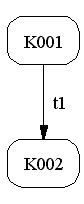
\includegraphics[height=0.5\textwidth]{Bilder/36_Verklemmung_KG_Graph.png}
	\caption{EG des Netzes mit Verklemmung}
	\label{fig:VKGG}
\end{minipage}
\end{figure}
\begin{figure}
\begin{minipage}[hbt]{7cm}
	\centering
	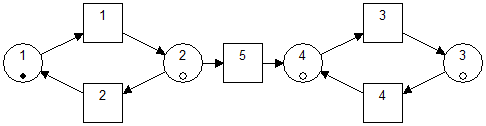
\includegraphics[width=0.7\textwidth]{Bilder/36_keine_Verklemmung_KG_Netz.png}
	\caption{Netz ohne Verklemmung}
	\label{fig:nVKGN}
\end{minipage}
\hfill
\begin{minipage}[hbt]{7cm}
	\centering
	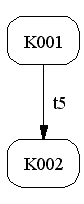
\includegraphics[height=0.5\textwidth]{Bilder/36_keine_Verklemmung_KG_Graph.png}
	\caption{EG des Netzes ohne Verklemmung}
	\label{fig:nVKGG}
\end{minipage}
\end{figure}

\end{enumerate}

\section{Aufgabe 2}

\subsection{Lebendigkeit}
Da bei der Übertragung beliebig viele Nachrichten verloren gehen können, muss dafür gesorgt werden, dass das zu erstellende Netz lebendig ist. Dadurch wird sichergestellt, dass alle Transition aus allen Markierungen heraus irgendwann einem schalten können, da für die Lebendigkeit gilt: $\forall t \in T : \text{t ist M-erreichbar}$. Das Netz darf bei einem Nachrichtenverlust nicht aufhören Nachrichten zu senden, solange bis die Bestätigungsnachricht mit dem invertieren Kontrollbit ankommt.

\subsection{Verklemmungsfreiheit}
Das Protokoll gibt einen strikten Ablauf vor, in dem  keine Zustände vorgesehen sind in denen nichts getan wird. Somit muss bei der Modellierung drauf geachtet werden, dass das Netz verklemmungsfrei ist. Das Protokoll definiert kein Ende ´"wiederholt diese solange, bis er vom Sender eine Nachricht mit dem anderen Bit, also das nächste Paket erhält"' wodurch es keinen Zustand geben darf in dem keine Transition mehr aktiv ist.

\subsection{Reversibilität}
Das Protokoll arbeitet mit einem invertierten Bit zur Kennzeichnung der Nachrichten. Da ein Bit nur zwei Werte annehmen kann, muss irgendwann der Ausgangszustand wieder hergestellt werden, an dem der Sender wieder anfängt Nachrichten mit dem Bit zu senden, welches er auch zum Anfang hatte.


\end{document}

